\documentclass[tikz]{standalone}
% \usepackage{tikz} % already loaded by the documentclass


\begin{document}
\centering
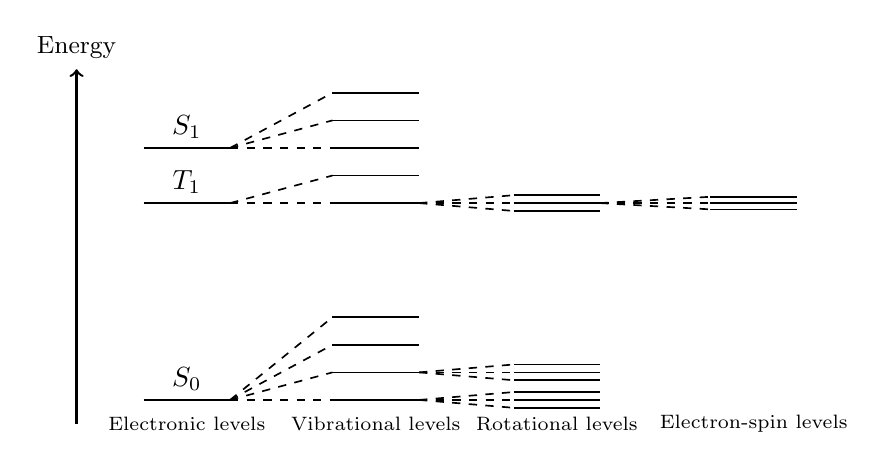
\begin{tikzpicture}[x=1cm,y=1cm,baseline]
% ----- columns (x) & rows (y) -----
\def\xElec{1.4}
\def\xVib{3.8}
\def\xRot{6.1}
\def\xSpin{8.6}

\def\ySone{3.50}
\def\yTone{2.80}
\def\ySzero{0.30}

% half-widths
\def\wElec{0.55}
\def\wVib{0.55}
\def\wRot{0.55}
\def\wSpin{0.55}

% spacings
\def\dvib{0.35}   % vibrational spacing (wide)
\def\drot{0.10}   % rotational spacing (= dvib/3)
\def\dspin{0.08}  % electron-spin spacing around center

% styles
\tikzset{lev/.style={line width=0.6pt}, dlev/.style={line width=0.6pt,dashed}}

% ----- axis -----
\draw[->,line width=0.9pt] (0,0) -- (0,4.5) node[above]{\small Energy};

% ===== S1 row =====
\draw[lev] (\xElec-\wElec,\ySone) -- (\xElec+\wElec,\ySone);
\node[above] at (\xElec,\ySone) {$S_1$};

% vib: 3 levels
\draw[lev] (\xVib-\wVib,\ySone+0*\dvib) -- (\xVib+\wVib,\ySone+0*\dvib);
\draw[lev] (\xVib-\wVib,\ySone+1*\dvib) -- (\xVib+\wVib,\ySone+1*\dvib);
\draw[lev] (\xVib-\wVib,\ySone+2*\dvib) -- (\xVib+\wVib,\ySone+2*\dvib);

% bridges S1→vib (3 lines; left at electronic right end, right at vib left end)
\draw[dlev] (\xElec+\wElec,\ySone) -- (\xVib-\wVib,\ySone+0*\dvib);
\draw[dlev] (\xElec+\wElec,\ySone) -- (\xVib-\wVib,\ySone+1*\dvib);
\draw[dlev] (\xElec+\wElec,\ySone) -- (\xVib-\wVib,\ySone+2*\dvib);

% ===== T1 row =====
\draw[lev] (\xElec-\wElec,\yTone) -- (\xElec+\wElec,\yTone);
\node[above] at (\xElec,\yTone) {$T_1$};

% vib: 2 levels (v0, v1)
\draw[lev] (\xVib-\wVib,\yTone+0*\dvib) -- (\xVib+\wVib,\yTone+0*\dvib);
\draw[lev] (\xVib-\wVib,\yTone+1*\dvib) -- (\xVib+\wVib,\yTone+1*\dvib);

% bridges T1→vib (2 lines)
\draw[dlev] (\xElec+\wElec,\yTone) -- (\xVib-\wVib,\yTone+0*\dvib);
\draw[dlev] (\xElec+\wElec,\yTone) -- (\xVib-\wVib,\yTone+1*\dvib);

% rot (centered at v0): r=-1,0,+1
\draw[lev] (\xRot-\wRot,\yTone-1*\drot) -- (\xRot+\wRot,\yTone-1*\drot);
\draw[lev] (\xRot-\wRot,\yTone+0*\drot) -- (\xRot+\wRot,\yTone+0*\drot); % r=0
\draw[lev] (\xRot-\wRot,\yTone+1*\drot) -- (\xRot+\wRot,\yTone+1*\drot);

% bridges |T1,v0>→rot (3 lines)
\draw[dlev] (\xVib+\wVib,\yTone+0*\dvib) -- (\xRot-\wRot,\yTone-1*\drot);
\draw[dlev] (\xVib+\wVib,\yTone+0*\dvib) -- (\xRot-\wRot,\yTone+0*\drot);
\draw[dlev] (\xVib+\wVib,\yTone+0*\dvib) -- (\xRot-\wRot,\yTone+1*\drot);

% electron-spin (ONLY for T; centered at |T1,v0,r=0>)
\draw[lev] (\xSpin-\wSpin,\yTone-1*\dspin) -- (\xSpin+\wSpin,\yTone-1*\dspin);
\draw[lev] (\xSpin-\wSpin,\yTone+0*\dspin) -- (\xSpin+\wSpin,\yTone+0*\dspin); % ms=0 (center)
\draw[lev] (\xSpin-\wSpin,\yTone+1*\dspin) -- (\xSpin+\wSpin,\yTone+1*\dspin);

% bridge rot (r=0) → spin (ms=0)
\draw[dlev] (\xRot+\wRot,\yTone+0*\drot) -- (\xSpin-\wSpin,\yTone-1*\dspin);
\draw[dlev] (\xRot+\wRot,\yTone+0*\drot) -- (\xSpin-\wSpin,\yTone+0*\dspin);
\draw[dlev] (\xRot+\wRot,\yTone+0*\drot) -- (\xSpin-\wSpin,\yTone+1*\dspin);

% ===== S0 row =====
\draw[lev] (\xElec-\wElec,\ySzero) -- (\xElec+\wElec,\ySzero);
\node[above] at (\xElec,\ySzero) {$S_0$};

% vib: 4 levels (v0..v3)
\draw[lev] (\xVib-\wVib,\ySzero+0*\dvib) -- (\xVib+\wVib,\ySzero+0*\dvib);
\draw[lev] (\xVib-\wVib,\ySzero+1*\dvib) -- (\xVib+\wVib,\ySzero+1*\dvib);
\draw[lev] (\xVib-\wVib,\ySzero+2*\dvib) -- (\xVib+\wVib,\ySzero+2*\dvib);
\draw[lev] (\xVib-\wVib,\ySzero+3*\dvib) -- (\xVib+\wVib,\ySzero+3*\dvib);

% bridges S0→vib (4 lines)
\draw[dlev] (\xElec+\wElec,\ySzero) -- (\xVib-\wVib,\ySzero+0*\dvib);
\draw[dlev] (\xElec+\wElec,\ySzero) -- (\xVib-\wVib,\ySzero+1*\dvib);
\draw[dlev] (\xElec+\wElec,\ySzero) -- (\xVib-\wVib,\ySzero+2*\dvib);
\draw[dlev] (\xElec+\wElec,\ySzero) -- (\xVib-\wVib,\ySzero+3*\dvib);

% rot clusters at S0 for v=0 and v=1 (each: r=-1,0,+1)
% v=0 center
\draw[lev] (\xRot-\wRot,\ySzero-1*\drot) -- (\xRot+\wRot,\ySzero-1*\drot);
\draw[lev] (\xRot-\wRot,\ySzero+0*\drot) -- (\xRot+\wRot,\ySzero+0*\drot);
\draw[lev] (\xRot-\wRot,\ySzero+1*\drot) -- (\xRot+\wRot,\ySzero+1*\drot);
% v=1 center
\draw[lev] (\xRot-\wRot,\ySzero+1*\dvib-1*\drot) -- (\xRot+\wRot,\ySzero+1*\dvib-1*\drot);
\draw[lev] (\xRot-\wRot,\ySzero+1*\dvib+0*\drot) -- (\xRot+\wRot,\ySzero+1*\dvib+0*\drot);
\draw[lev] (\xRot-\wRot,\ySzero+1*\dvib+1*\drot) -- (\xRot+\wRot,\ySzero+1*\dvib+1*\drot);

% bridges from |S0,v0> and |S0,v1> only (6 lines total)
\draw[dlev] (\xVib+\wVib,\ySzero+0*\dvib) -- (\xRot-\wRot,\ySzero-1*\drot);
\draw[dlev] (\xVib+\wVib,\ySzero+0*\dvib) -- (\xRot-\wRot,\ySzero+0*\drot);
\draw[dlev] (\xVib+\wVib,\ySzero+0*\dvib) -- (\xRot-\wRot,\ySzero+1*\drot);
\draw[dlev] (\xVib+\wVib,\ySzero+1*\dvib) -- (\xRot-\wRot,\ySzero+1*\dvib-1*\drot);
\draw[dlev] (\xVib+\wVib,\ySzero+1*\dvib) -- (\xRot-\wRot,\ySzero+1*\dvib+0*\drot);
\draw[dlev] (\xVib+\wVib,\ySzero+1*\dvib) -- (\xRot-\wRot,\ySzero+1*\dvib+1*\drot);

% ----- category labels (restored) -----
\node[align=center,font=\scriptsize] at (\xElec,0.0) {Electronic levels};
\node[align=center,font=\scriptsize] at (\xVib,0.0) {Vibrational levels};
\node[align=center,font=\scriptsize] at (\xRot,0.0) {Rotational levels};
\node[align=center,font=\scriptsize] at (\xSpin,0.0) {Electron-spin levels};
\end{tikzpicture}
\end{document}
      